もし大きな文書、例えば100ページを越える書籍を作るような場合、テスト・コンパイルにrakeを使う(rakeで文書全体をコンパイルするという意味)のは良い方法ではない。
ドキュメントが大きくなればなるほど、コンパイル時間が長くなるからである。

それよりは、lbを使ってサブファイルを単独でコンパイルするのが良い方法である。
lbは一時的なルートファイル(テンポラリ・ルートファイルという)を作り、その中にサブファイルを取り込む命令を記述し、1度だけコンパイルする。
この方法の良い点は短時間でコンパイルできることである。
しかし、良くない点もある。
サブファイルのみのコンパイルであるから、文書全体のpdfを見ることはできない。
また、1度だけのコンパイルなので、相互参照は反映されない。
どちらが良いかは一概には言えない。
それは作成している文書によるが、もしそれが非常に大きな文書であれば、テスト・コンパイルをlbでやるほうがより良いといえる。

次のようにタイプしてほしい。
\begin{verbatim}
$ lb installation
\end{verbatim}
この引数はサブファイル名である。
拡張子は省略することもできる。

すると、lbはテンポラリ・ルートファイル「\_build/test\_installation.tex」を作る。
そのプリアンブルは元のルートファイルのプリアンブルのコピーである。
そして、{\textbackslash}inputコマンドでサブファイルの「installation.tex」を取り込むようになっている。
lbは「\_build/test\_installation.tex」をコンパイルし、lb.confで指定されたpdfビューワを起動してpdfファイルを表示する。
\begin{center}
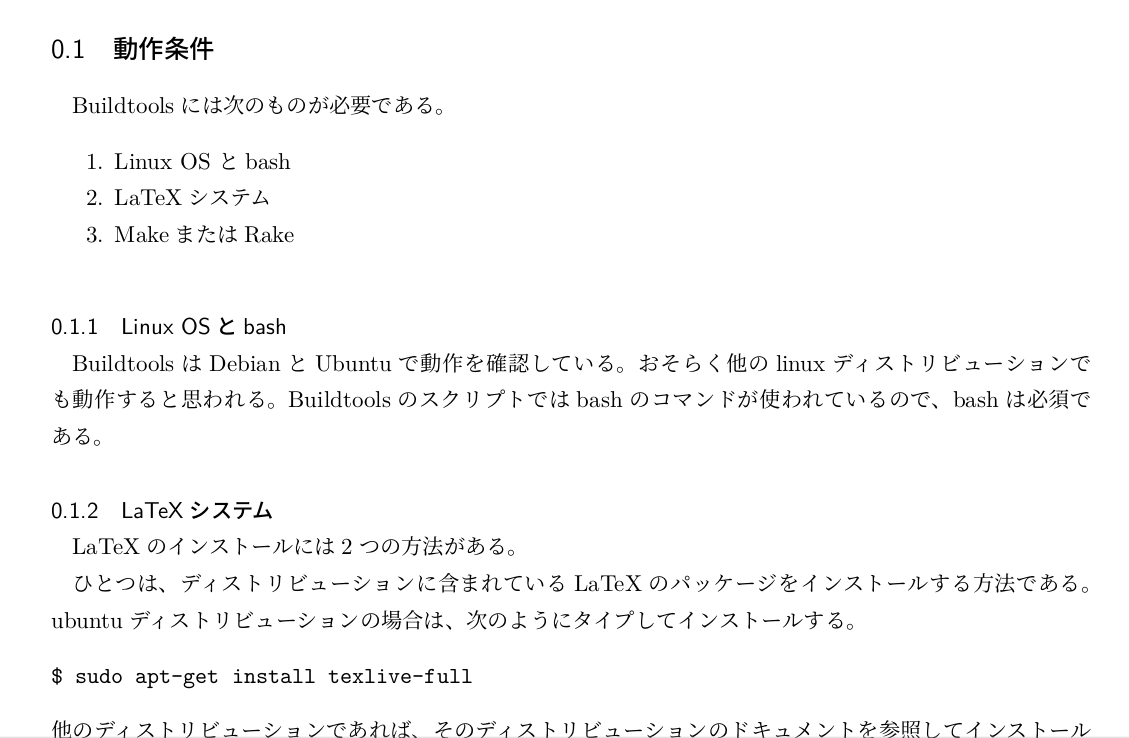
\includegraphics[width=12cm]{test_installation.png}
\end{center}

lbはコンパイルするときにsynctexのオプションをオンにする。
したがって、ソースファイルの「\_build/test\_installation.tex」と「installation.tex」をエディタで開いておけば、ソースとpdfの間で前方参照と後方参照をすることができる。
もしもgeditをエディタに、evinceをビューワに使っていれば、コントロール・キーを押したまま左クリックすれば後方参照(pdfからソースへの参照)が可能である。
しかし、「installation.tex」からpdfへの前方参照は働かない。
それを機能させるためには、サブファイルの先頭に次の1行を加えなければならない。
\begin{verbatim}
% mainfile: _build/test_installation.tex
\end{verbatim}
しかし、前方参照を使うことは後方参照に比べそう多くはない。
上記の1行を加えるのは、たいていは必要ないだろう。

